\documentclass[11pt,a4paper]{article}
\usepackage[utf8]{inputenc}
\usepackage[T1]{fontenc}
\usepackage[margin=2.5cm]{geometry}
\usepackage{amsmath,amssymb}
\usepackage{graphicx}
\usepackage{booktabs}
\usepackage{hyperref}
\hypersetup{colorlinks=true, linkcolor=blue, urlcolor=blue, citecolor=blue}
\graphicspath{{../figures/}}

% Include a figure only if it has already been generated by the scripts.
\newcommand{\optfig}[3]{%
  \IfFileExists{../figures/#1}{%
    \begin{figure}[h]\centering
      \includegraphics[width=#2\textwidth]{#1}
      \caption{#3}\end{figure}}{%
    \begin{quote}\itshape[Figure \texttt{\detokenize{#1}} is generated by the study scripts;
      run scripts/run\_study.py to produce it.]\end{quote}}}

\title{\textbf{What Does LoRA Change?}\\
\large An interpretability study of Low-Rank Adaptation in a small LLM}
\author{Marcos Lahoz}
\date{}

\begin{document}
\maketitle

\begin{abstract}
Low-Rank Adaptation (LoRA) fine-tunes large language models by learning small
low-rank updates to frozen weight matrices. It is ubiquitous, yet it is rarely
asked \emph{what} a LoRA adapter actually changes inside the model. We study this
on \texttt{Qwen2.5-1.5B} instruction-tuned on Alpaca, with two complementary,
training-free diagnostics: (i) the \emph{relative update magnitude}
$\lVert\Delta W\rVert/\lVert W\rVert$ and the effective rank of $\Delta W$ for
every adapted projection, revealing where LoRA concentrates its capacity; and
(ii) the \emph{representation drift} between the adapter-enabled and
adapter-disabled model, layer by layer, revealing how far the internal
representations move and at what depth. We run these across an ablation over the
LoRA rank and the set of adapted modules. We then test whether the findings
\emph{generalise}: we repeat the diagnostics on a second model family
(\texttt{SmolLM2-1.7B}) and a second PEFT variant (DoRA), with two upgrades ---
\emph{exact} update norms measured by merging the adapter and diffing against the
base weights, and a \emph{behavioural validation} via held-out instruction loss.
The first three findings replicate. The fourth becomes a sharper, DoRA-specific
result: reading DoRA's learned magnitude vector into the exact update shows that
DoRA matches LoRA in update \emph{magnitude} and in its effect on representations,
yet writes that change into a far \emph{higher-rank} weight perturbation
(participation ratio $\approx 540$/$1281$ vs.\ $\approx 13$/$10$ for LoRA). The
magnitude component, not the direction, is what distinguishes DoRA in weight
space. The framework turns ``LoRA works'' into measurable, localised statements
about a fine-tuned model.
\end{abstract}

\section{Introduction}
LoRA~\cite{hu2021lora} freezes a pretrained weight $W\in\mathbb{R}^{d_\text{out}\times d_\text{in}}$
and learns a low-rank update $\Delta W=\tfrac{\alpha}{r}BA$ with
$B\in\mathbb{R}^{d_\text{out}\times r}$, $A\in\mathbb{R}^{r\times d_\text{in}}$ and
$r\ll d$. It is the default way to fine-tune LLMs cheaply, but it is usually
treated as a black box. We ask three questions:
\begin{enumerate}
  \item \textbf{Where} does LoRA put its capacity --- which layers and which
        projection types ($q,k,v,o$ vs. the MLP $\text{gate},\text{up},\text{down}$)
        receive the largest updates?
  \item \textbf{How much} do the model's hidden representations actually move
        once the adapter is enabled, and at which depth?
  \item How do (1) and (2) depend on the LoRA \textbf{rank} and the set of
        \textbf{adapted modules}?
\end{enumerate}
The analyses are training-free post-hoc diagnostics and apply to any
LoRA-adapted transformer.

\section{Method}
\paragraph{(1) Effective update magnitude.} For each adapted module we form the
explicit update $\Delta W=\tfrac{\alpha}{r}BA$ and report the relative Frobenius
norm
\[
  \rho \;=\; \frac{\lVert \Delta W\rVert_F}{\lVert W\rVert_F},
\]
i.e. how large the change is compared with the original weight. We also summarise
the \emph{shape} of $\Delta W$ by the participation ratio of its singular values
$\{\sigma_i\}$,
\[
  \text{eff-rank}(\Delta W) \;=\; \exp\!\Big(-\sum_i p_i\log p_i\Big),\qquad
  p_i=\frac{\sigma_i}{\sum_j\sigma_j},
\]
which measures how many directions the update effectively uses. For a low-rank
$\Delta W=\tfrac{\alpha}{r}BA$ this is bounded by $r$; for the \emph{exact} merged
update of DoRA (\S\ref{sec:generality}) it need not be, since the magnitude
rescaling acts on the full-rank base weight.

\paragraph{(2) Representation drift.} Let $h^{(\ell)}_{\text{on}}(x)$ and
$h^{(\ell)}_{\text{off}}(x)$ be the mean-pooled hidden state at layer $\ell$ for
input $x$ with the adapter enabled and disabled (the rest of the model is
identical). Over a held-out set $\mathcal{X}$ we report, per layer, the mean
cosine similarity and the relative $L_2$ drift
\[
  \text{cos}^{(\ell)} = \tfrac{1}{|\mathcal X|}\!\sum_{x}\!\cos\big(h^{(\ell)}_{\text{on}},h^{(\ell)}_{\text{off}}\big),
  \qquad
  \delta^{(\ell)} = \tfrac{1}{|\mathcal X|}\!\sum_{x}\!\frac{\lVert h^{(\ell)}_{\text{on}}-h^{(\ell)}_{\text{off}}\rVert}{\lVert h^{(\ell)}_{\text{off}}\rVert}.
\]
This isolates the causal effect of the adapter on the representations.

\section{Experimental setup}
We fine-tune the base \texttt{Qwen2.5-1.5B} on a subset of Alpaca with an
instruction template, training only the LoRA adapters. We ablate the rank
$r\in\{4,16,64\}$ and the adapted module set
(\textit{attn}: $q,k,v,o$; \textit{all}: $+\,\text{gate},\text{up},\text{down}$).
Representation drift is measured on a fixed set of held-out instructions. All
code, the ablation runner and the plots are in the repository.

\section{Results}
We fine-tune for one epoch on 2{,}000 Alpaca examples per configuration. Training
converges to a similar loss everywhere (1.39--1.47), with only small gains from
larger rank or adapting all modules (best: rank~64, all, train loss~1.41),
already hinting at \emph{diminishing returns}. Table~\ref{tab:abl} and
Figure~\ref{fig:summary} summarise the diagnostics.

\begin{table}[h]\centering
\begin{tabular}{llrrrrr}
\toprule
rank & modules & mean $\rho$ & $\rho$(attn) & $\rho$(mlp) & eff-rank($\Delta W$) & drift (rel.\,$L_2$) \\
\midrule
4  & attn & 0.0063 & 0.0063 & --     & 3.24  & 0.299 \\
16 & attn & 0.0088 & 0.0088 & --     & 11.77 & 0.320 \\
64 & attn & 0.0145 & 0.0145 & --     & 44.90 & 0.314 \\
4  & all  & 0.0039 & 0.0042 & 0.0035 & 3.55  & 0.250 \\
16 & all  & 0.0063 & 0.0069 & 0.0056 & 13.41 & 0.257 \\
64 & all  & 0.0117 & 0.0127 & 0.0104 & 52.01 & 0.224 \\
\bottomrule
\end{tabular}
\caption{Ablation summary. $\rho=\lVert\Delta W\rVert/\lVert W\rVert$ averaged over
adapted modules; eff-rank is the participation ratio of $\Delta W$'s singular
values; drift is the final-layer relative-$L_2$ representation drift.}
\label{tab:abl}
\end{table}

\begin{figure}[h]\centering
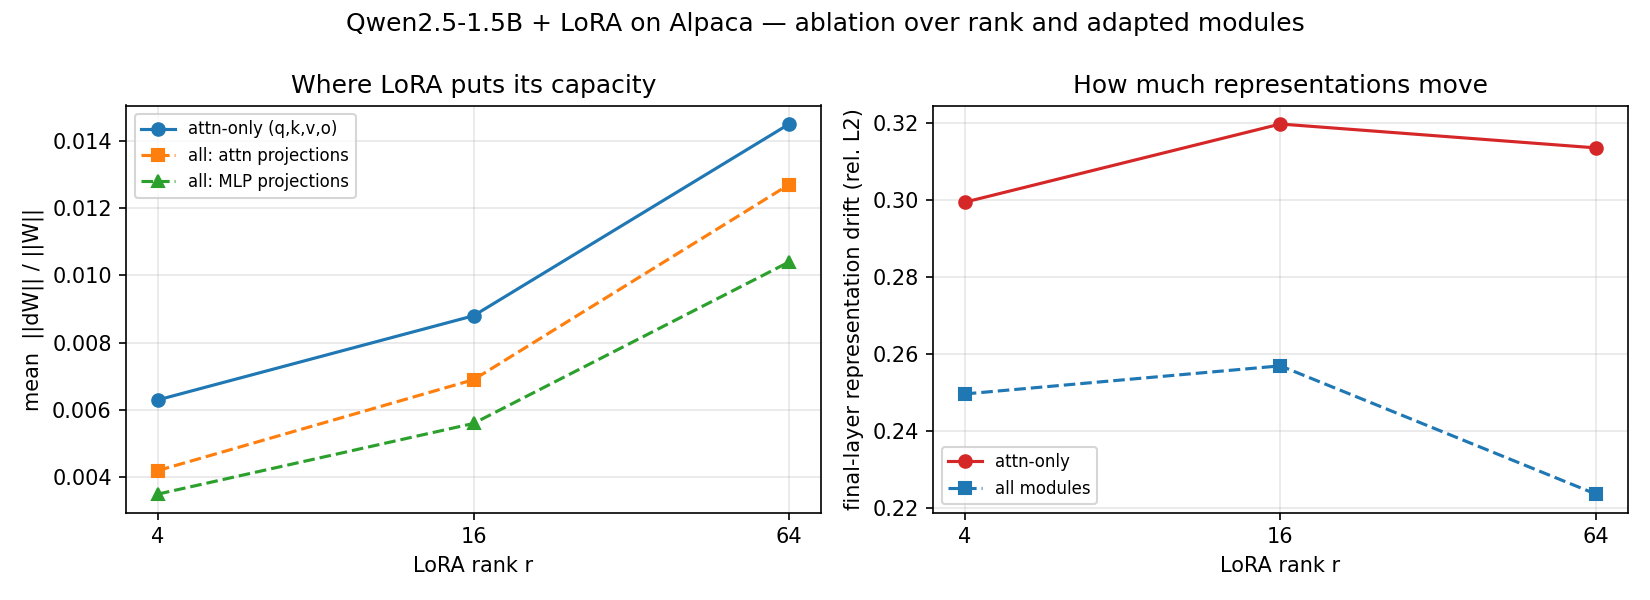
\includegraphics[width=0.95\textwidth]{summary_ablation.png}
\caption{Left: relative update magnitude grows with rank, and attention
projections receive larger updates than the MLP. Right: final-layer
representation drift; adapting all modules moves representations less than
attention-only at matched rank.}
\label{fig:summary}
\end{figure}

Four findings stand out:
\begin{enumerate}
  \item \textbf{Updates are tiny in magnitude.} $\rho$ stays around
        $0.4\%$--$1.5\%$: LoRA makes small, targeted edits to the weights rather
        than large changes.
  \item \textbf{LoRA uses (almost) its full rank budget.} The effective rank of
        $\Delta W$ tracks $r$ closely (3.2 at $r{=}4$, 11.8 at $r{=}16$, $\sim$45--52
        at $r{=}64$): the adaptation is genuinely high-dimensional, not a rank-1
        shortcut.
  \item \textbf{Attention changes more than the MLP.} Under the \textit{all}
        setting, attention projections consistently receive larger relative
        updates than the MLP across every rank.
  \item \textbf{Fine-tuning rescales rather than rotates representations.}
        Final-layer cosine similarity between the adapter-on and adapter-off model
        stays high ($0.96$--$0.98$) while the relative-$L_2$ drift is sizeable
        ($0.22$--$0.32$): the \emph{direction} of the representations is largely
        preserved, but their \emph{magnitude/offset} moves. Spreading capacity
        across all modules yields lower per-layer drift than attention-only at the
        same rank.
\end{enumerate}
Together with the near-flat training loss across ranks, this indicates that for
this model/task a small rank already captures most of the adaptation, and the
extra capacity of large ranks is only partly used.

\section{Generality: a second model family and DoRA}
\label{sec:generality}

The ablation above is a single-model, single-variant study. To test whether its
conclusions are properties of \emph{LoRA fine-tuning} rather than of
\texttt{Qwen2.5-1.5B}, we repeat the diagnostics at rank~16 (\textit{all}
modules, same data and budget) along two new axes: a second model family,
\texttt{SmolLM2-1.7B} (a Llama-style architecture), and a second PEFT variant,
\textbf{DoRA}~\cite{dora}, which decomposes the update into a magnitude and a
direction component.

Two methodological upgrades accompany the extension. First, update norms are
now \emph{exact}: we snapshot the frozen base weights, merge the trained
adapter, and measure $\Delta W$ as the difference of the merged and base
matrices --- for DoRA, the $(\alpha/r)\,BA$ formula would miss the magnitude
component, whereas the merge-and-diff measurement includes it. Second, every
configuration passes a \emph{behavioural validation} before its weights are
interpreted: mean token-level cross-entropy on 200 held-out Alpaca examples,
base vs.\ fine-tuned, so the diagnostics are guaranteed to describe runs that
actually adapted.

\begin{table}[h]\centering
\small
\begin{tabular}{llcrrrrrr}
\toprule
model & variant & loss (base$\to$ft) & mean $\rho$ & $\rho$(attn) & $\rho$(mlp) & eff-rank & drift cos & drift $L_2$ \\
\midrule
Qwen2.5-1.5B & LoRA & $1.97\to1.45$ & 0.0063 & 0.0069 & 0.0056 & 13.4 & 0.971 & 0.257 \\
Qwen2.5-1.5B & DoRA & $1.97\to1.45$ & 0.0066 & 0.0071 & 0.0060 & \textbf{540.5} & 0.971 & 0.259 \\
SmolLM2-1.7B & LoRA & $2.23\to1.37$ & 0.0022 & 0.0023 & 0.0020 & 10.2 & 0.927 & 0.375 \\
SmolLM2-1.7B & DoRA & $2.23\to1.37$ & 0.0028 & 0.0029 & 0.0027 & \textbf{1280.9} & 0.928 & 0.373 \\
\bottomrule
\end{tabular}
\caption{Generality study (rank 16, all modules, 2{,}000 Alpaca examples, one
epoch). Update norms are exact (merge-and-diff), reading DoRA's learned magnitude
vector so its magnitude component is included in $\Delta W$. Every configuration
improves held-out instruction loss by $0.5$--$0.9$ nats before being interpreted.}
\label{tab:gen}
\end{table}

The first three findings replicate on the second family
(Table~\ref{tab:gen}): updates remain tiny (mean $\rho\le 0.7\%$ for both LoRA
and DoRA; SmolLM2 is even more frugal at $\approx 0.2$--$0.3\%$); for LoRA most
of the rank budget is used ($13.4/16$ on Qwen, $10.2/16$ on SmolLM2 ---
substantial but model-dependent); attention receives larger relative updates
than the MLP in all four configurations; and the rescale-not-rotate signature
persists (final-layer cosine $0.97/0.93$ with sizeable relative-$L_2$ drift
$0.26/0.37$ --- SmolLM2 moves direction somewhat more than Qwen). LoRA and DoRA
drift almost identically: their \emph{behavioural} effect is the same.

\paragraph{A new finding: DoRA differs from LoRA in the rank of the update, not
its magnitude.} Update magnitude, attention bias and representation drift all
match between LoRA and DoRA within noise --- but the \emph{effective rank} of the
merged update does not. For LoRA the exact $\Delta W$ is genuinely low-rank,
tracking the budget $r$ (participation ratio $13.4$ on Qwen, $10.2$ on SmolLM2).
For DoRA the exact $\Delta W$ is \emph{high-rank} --- $\approx 540$ on Qwen and
$\approx 1281$ on SmolLM2 --- because the per-row magnitude rescaling
$m\cdot(W_0+\Delta V)/\lVert W_0+\Delta V\rVert_{\text{row}}$ acts on the
full-rank base weight, spreading $\Delta W$ across hundreds of directions even
though DoRA's \emph{trainable} directional component is still rank $\le r$. This
difference is invisible to the directional $(\alpha/r)\,BA$ estimator and appears
only once the magnitude component is measured. So at this scale and task LoRA and
DoRA are indistinguishable in update magnitude and in their effect on
representations, yet DoRA writes that same change into a much higher-rank weight
perturbation. Whether this higher-rank footprint translates into a behavioural
advantage at larger scale or on tasks where DoRA reports gains is an open
question the framework can answer directly.

\section{Discussion and future work}
The two diagnostics localise fine-tuning: $\rho$ shows which weights move, the
effective rank shows how low-dimensional the change is, and the drift curve shows
where in the network behaviour is reshaped (typically the later layers). The generality study
(Section~\ref{sec:generality}) shows these are statements about LoRA-style
fine-tuning, not about one model, and that DoRA leaves update magnitude and
representation drift unchanged while writing a far higher-rank weight
perturbation --- a difference only the exact, magnitude-aware diagnostic reveals.
Natural extensions: (i) scaling the grid to 7B+ models and longer training,
where DoRA's reported gains might translate into diagnostic differences;
(ii) trained linear \emph{probes} on the representations before/after,
connecting to structural-probe methodology; (iii) tracking weight-space
directions of the merged updates across tasks.

\begin{thebibliography}{9}
\bibitem{hu2021lora} Hu, E. et al. (2021). \emph{LoRA: Low-Rank Adaptation of Large Language Models}. arXiv:2106.09685.
\bibitem{dora} Liu, S.-Y. et al. (2024). \emph{DoRA: Weight-Decomposed Low-Rank Adaptation}. ICML.
\bibitem{hewitt2019} Hewitt, J. \& Manning, C. (2019). \emph{A Structural Probe for Finding Syntax in Word Representations}. NAACL.
\bibitem{qwen} Qwen Team (2024). \emph{Qwen2.5 Technical Report}.
\end{thebibliography}
\end{document}
